\documentclass[aps,pre,preprint]{revtex4}
% \documentclass[aps,pre,twocolumn]{revtex4-1}
% \documentclass[aps,jcp,groupedaddress,twocolumn,unsortedaddress]{revtex4}

\usepackage{amsmath}
\usepackage{amssymb}
\usepackage[dvips]{graphicx}
\usepackage{color}
\usepackage{tabularx}

\makeatletter
\makeatother

\newcommand{\recheck}[1]{{\color{red} #1}}
\newcommand{\redc}[1]{{\color{red} #1}}
\newcommand{\bluec}[1]{{\color{blue} #1}}
\renewcommand{\v}[1]{\textbf{\textit{#1}}}
\renewcommand{\d}[1]{\textsf{#1}}


\begin{document}

% \title{The Error Estimate of Force Calculation in the Inhomogeneous Molecular Systems}
% \author{Han Wang}
% \affiliation{LMAM and School of Mathematical
%   Sciences, Peking University}
% \author{Pingwen Zhang}
% % \email{pzhang@pku.edu.cn}
% \affiliation{LMAM and School of Mathematical
%   Sciences, Peking University}

% \begin{abstract}
% \end{abstract}

% \maketitle

\begin{figure}
  \centering
  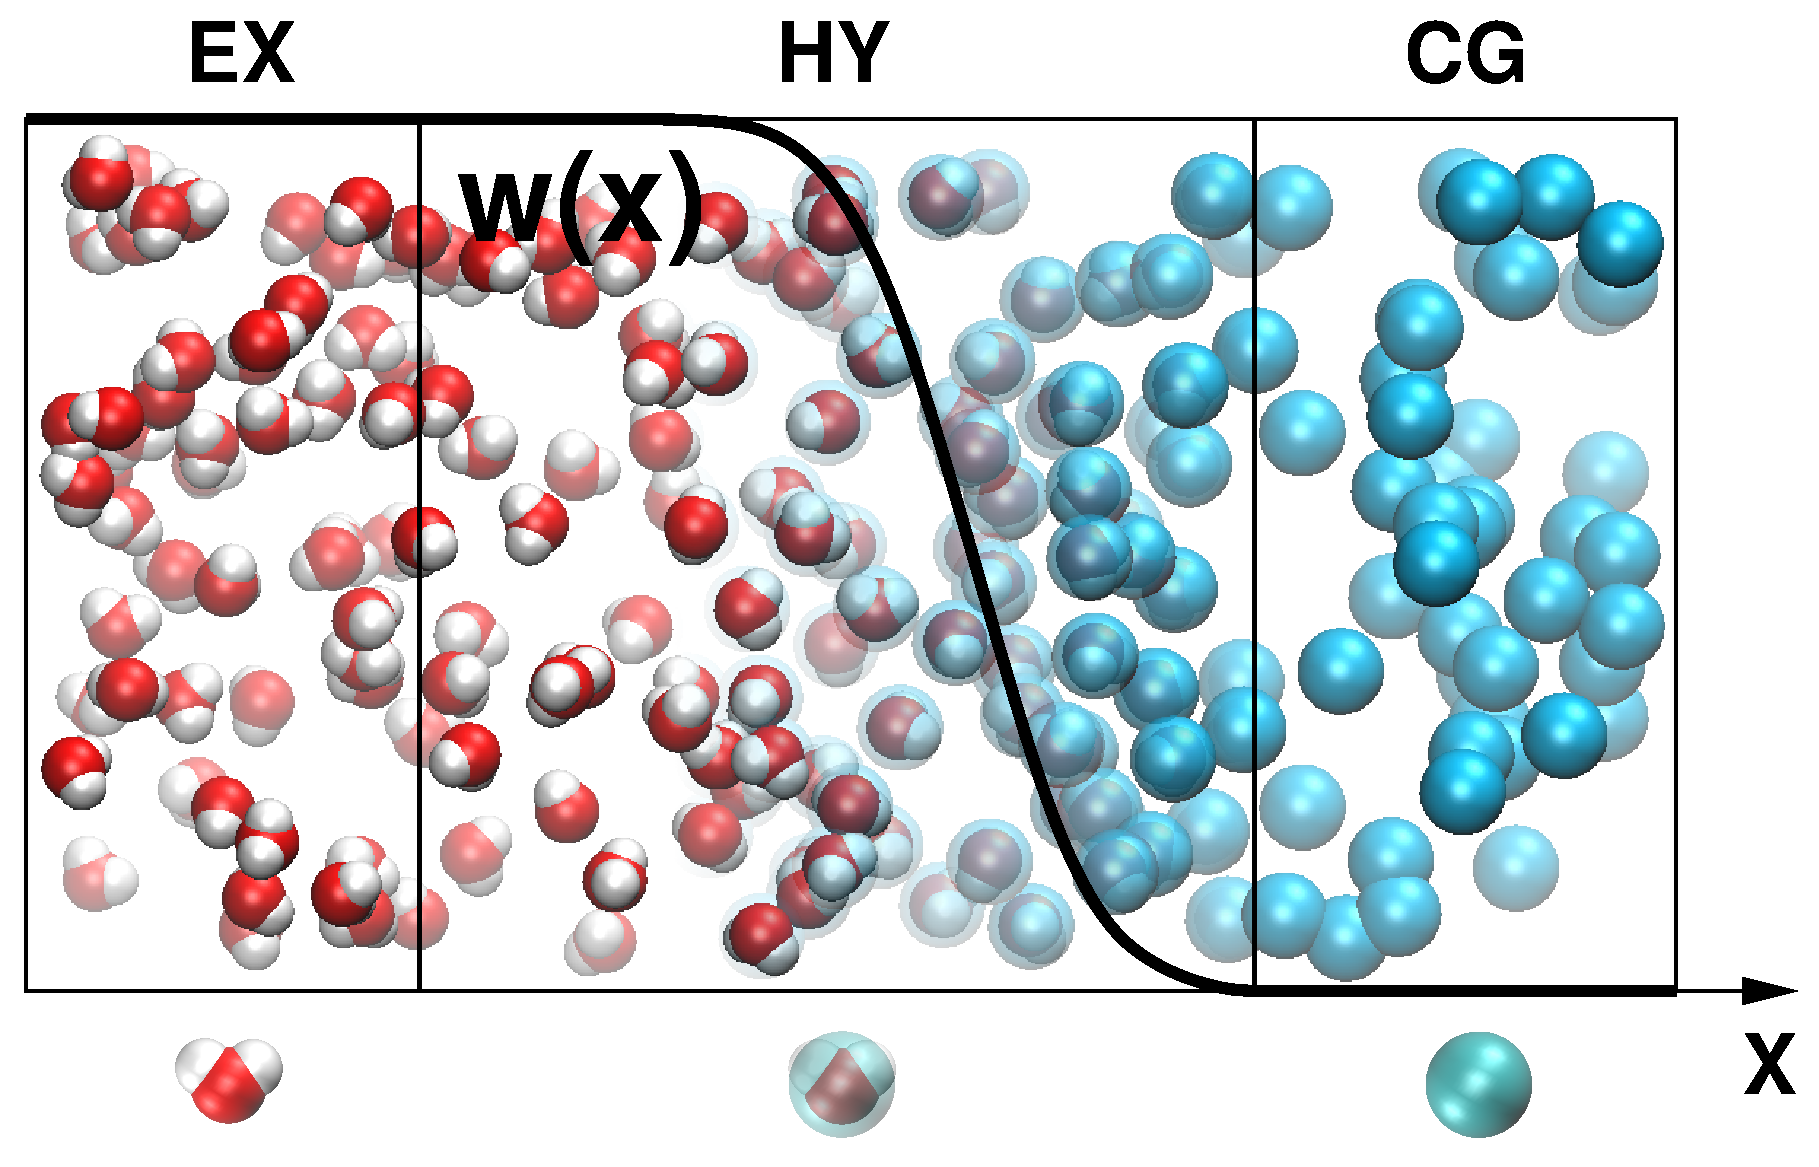
\includegraphics[width=.5\textwidth]{fig/system.eps}
  \caption{An AdResS system}
  \label{fig:tmp1}
\end{figure}


We want to prove the trajactory of the explicit region in Adress
simulation is an implementation of the $\mu$VT distribution. We take a
sequency of snapshots of the system along the trajactory.  For sure,
the number of molecules in the explicit region varies. We group the
snapshots by the number of molecules in the explicit region.  The
stratagy of our provment is firstly to shown the position and
velocity distribution in each group, where the number of molecules
in the explicit region is fixed, is subject to the Boltzmann
distribution. Secondly, we show the number of snapshots in each group
is subject to the exponential distribution. Then the combination of
these two distributions ends up with the grand-canonical distribution.

Notice, the prove always compare the explicit region to an sub-system
of a big all-atom canonical system. If the explicit region is embeded
into the whole Adress system in the same maner as the sub-system
embeded in to the big all-atom canonical system, then the Adress will
give the correct grand-canonical distribution.

\section{Embeded explicit region}

Consider the dynamics of a system that is subject to the Langevin equation:
\begin{align}
  \d d\v r_i &= \v v_i\d dt\\
  m_i\d d\v v_i &= [-m_i\xi_i\v v_i + \v F_i]\,\d dt + \sqrt{2\sigma_i}\,\d d\v W_t
\end{align}
where $\d d\v W_t$ is the standard Wiener process.  If the system has a
potential, namely $\v F_i = -\nabla_{\v r_i}U$, then it can be proved that the
Langevin dynamics generates the canonical ensemble:
\begin{align}
  p(\v r_1, \cdots, \v r_N, \v v_1, \cdots, \v v_N)
  = \exp\big[
  -\beta \mathcal H(\v r_1, \cdots, \v r_N, \v v_1, \cdots, \v v_N)
  \big]
  % \bigg[
  % \sum_i^N\frac12 m_i\v v_i^2 + U(\v r_1, \cdots, \v r_N)
  % \bigg]
\end{align}
where $\mathcal H$ is the Hamiltonian of the system:
\begin{align}
  \mathcal H(\v r_1, \cdots, \v r_N, \v v_1, \cdots, \v v_N)
  =
  \sum_{i=1}^N\frac12 m_i\v v_i^2 + U(\v r_1, \cdots, \v r_N)  
\end{align}

For the Adress simulation, let us first consider there are $N_1$
molecules in the explicit region, $N_2 - N_1$ molecules in the hybrid
region.  Without lost of generalty, we assume molecules $1, \cdots,
N_1$ are in the explicit region, molecules $N_1 + 1, \cdots, N_2$ are
in the hybrid region and $N_2+1, \cdots, N$ are in the coarse-grained
region. The pair $\{\v r_i, \v v_i\}$ of the explicit representation
denotes the center-of-mass (COM) position and velocity of the $i$-th
molecule. For convenience, we only consider the COM coordinate of the
explicit molecule, all the prove can be easily extended to treat every
atom the the molecule.

We hereby consider the explicit region as a sub-system of the whole
system, which composes the explicit, hybrid and coarse-grained
regions. We want to prove that the explicit region can be viewed as a
$\mu$VT sub-system, which is embeded into a huge NVT environment.
For any molecule $i$ in the explicit region, the force exerting on
it is
\begin{align}
  \v F_i &= \sum_{j=1}^{N}\v F_{ij} 
  =
  \sum_{j=1}^{N_1}\v F_{ij} + \sum_{j=N_1+1}^{N_2}\v F_{ij} 
\end{align}
Here it is assumed that the width of the hybrid region is larger than
the cut-off of the pairwise interaction $\v F_{ij}$, so the molecule
in the explicit region is not interacting with the molecules in the
coarse-grained region, as this happens in all applications.
The Adress force interpolation scheme reads:
\begin{align}\label{eqn:f-interp}
  \v F_{ij} = w_iw_j\v F^{\textrm{ex}}_{ij} + [1-w_iw_j]\v F^{\textrm{cg}}_{ij},
\end{align}
where $w_i = w(\v r_i)$ represents
the resolution of the molecule:
\begin{align}\label{eqn:w1}
  w(\v r) =
  \left\{
    \begin{array}{lcl}
      1 &\quad& \textrm{atomistic region}\\
      0<w<1  && \textrm{hybrid region}\\
      0 && \textrm{coarse-grained region}.
    \end{array}
  \right.
\end{align}
Specifically, we have the weighting function:
\begin{align}\label{eqn:w2}
  w(\v r) =
  \left\{
    \begin{array}{lcl}
      1 &\quad& \chi < d_{\textrm{ex}}\\
      1  && d_{\textrm{ex}} < \chi < d_{\textrm{ex}} + r_c\\
      \cos^2\big[\frac{\pi}{2(d_{\textrm{hy}} - r_c)} (\chi - d_{\textrm{ex}} - r_c)\big] && d_{\textrm{ex}} + r_c < \chi < d_{\textrm{ex}} + d_{\textrm{hg}} \\
      0 && d_{\textrm{ex}} + d_{\textrm{hg}}  < \chi.
    \end{array}
  \right.
\end{align}
Where $d_{\textrm{ex}}$ and $d_{\textrm{hy}}$ are the size of the
explicit and hybrid region, respectively. $r_c$ is the cut-off
radius. Here $d_{\textrm{hy}} \geq 2r_c$. $\chi$ is the distance to
the border of the explicit region.  The molecules in the hybrid region
is applied a thermodynamic force $\v F^{\textrm{th}}(\v x)$
\begin{align}
  \v F_i = \sum_j\v F_{ij} + \v F^{\textrm{th}}(\v x_i),
\end{align}
which is defined to ensure a uniform grand potential:
\begin{align}
  \bigg(
  p(\v x_0) +
  \frac{\rho}{M}\int_{\v x_0}^{\v x_1}\v F^{\textrm{th}}(\v s)\,\d d\v s
  \bigg) V
  =
  p(\v x_1) V
\end{align}
From thermodynamic point of view, the thermodynamic force will lead
to the same chemical potential for the explicit and coarse-grained regions.
% This definition of $w(\v r)$ is \emph{different from the convention}, which
% has a value of 1 for the atomistic region and 0 for the coarse-grained
% region.

By the definition of the force interpolation scheme
\eqref{eqn:f-interp} and \eqref{eqn:w2}, the interaction between the
explicit molecules and hybrid molecules is
\begin{align}
  \v F_{ij} = \v F^{\textrm{ex}}_{ij}
\end{align}
and obviously in the explicit region
\begin{align}
  \v F_i =
  \sum_{j=1}^{N_1}\v F^{\textrm{ex}}_{ij} + \sum_{j=N_1+1}^{N_2}\v F^{\textrm{ex}}_{ij}, \quad 1\leq i \leq N_1
\end{align}
Therefore, if we fix the coordinates of the molecules in the hybrid
region, the Hamiltonian of the explicit region can be written as
\begin{align}
  \mathcal H^{\textrm{ex}}(\v x_1; \v x_2) =
  \sum_{j=1}^{N_1}\frac12 m_i\v v_i^2 + 
  \sum_{i,j=1}^{N_1}\frac12 U^{\textrm{ex}}(\v r_i - \v r_j) + 
  \sum_{i=1}^{N_1}\sum_{j=N_1+1}^{N_2} U^{\textrm{ex}}(\v r_i - \v r_j) 
\end{align}
We denote the phase space variables: $\v x_1 = (\v r_1, \cdots, \v
r_{N_1}, \v v_1, \cdots, \v v_{N_1})$,  $\v x_2 = (\v r_{N_1+1},
\cdots, \v r_{N_2}, \v v_{N_1+1}, \cdots, \v v_{N_2})$ and
$\v x_3 = (\v r_{N_2+1},
\cdots, \v r_{N_3}, \v v_{N_2+1}, \cdots, \v v_{N_3})$.
Here $\v x_1$ is the variable and $\v x_2$ is considered as environment, 
by the Langevin dynamics, we have the conditional probability distribution
\begin{align}
  p (\v x_1 \vert \v x_2)  =
  e^{-\beta \mathcal H^{\textrm{ex}}(\v x_1; \v x_2)}
\end{align}
The phase space distribution of the explicit region:
\begin{align}
  p(\v x_1) = \int p(\v x_1\vert\v x_2)\cdot p (\v x_2) \,\d d\v x_2
\end{align}
If the phase space distribution $p(\v x_2)$ is the same as the explicit
Boltzmann distribution, then the explicit region is
equivalently embeded in to a explicit molecular environment and can be
viewed as a sub-system of a very big explicit molecular
system.

The crucial question is if $p(\v x_2)$ is correct.  A necessary
condition is that both the density and the radial distribution
function (RDF) are correct in the hybrid region. By the thermodynamic
force correction, the density is correct. Now the RDF...  If the
coarse-grained potential is generated by fitting the explicit RDF,
\redc{then in the hybrid region, it seems the RDF should not deviate very
  far from the correct.}

\begin{figure}
  \centering
  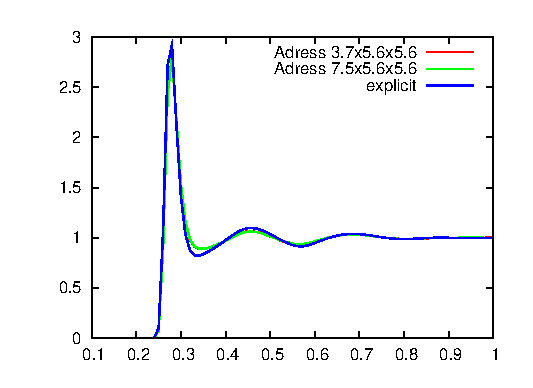
\includegraphics[]{fig/rdfs.eps}
  \caption{The RDF is independent with the size of the hybrid region.
    In the Adress simulation, the whole region is defined hybrid. They
    are compared with the explicit water RDF.}
  \label{fig:tmp2}
\end{figure}

\bluec{
  What we want to do next is
  \begin{itemize}
  \item Theoretically show under what kind of condition the RDF is
    correct.
  \item We find the current Adress scheme (with thermodynamic force
    applied) will not give perfect RDF in the hybrid region. However,
    the RDF profile is independent with the size of the hybrid region
    see Fig. \ref{fig:tmp2}. This fact gives rise to the idea of
    applying addtional correction force in the hybrid region to fit
    the RDF, a possible form is
    \begin{align}
      \v F_{ij} = w_iw_j\v F^{\textrm{ex}}_{ij} + [1-w_iw_j]\v F^{\textrm{cg}}_{ij} +
      4 w_iw_j (1 - w_iw_j)\v F_{ij}^{\textrm{rdf}},
    \end{align}
    notice the thermodynamic force should also be added
    \begin{align}
      \v F_i = \sum_j\v F_{ij} + \v F^{\textrm{th}}(\v x_i),
    \end{align}
    The correction force $\v F_{ij}^{\textrm{rdf}}$ that is only
    applied in the hybrid region can be obtained by the
    coarse-graining method that fits the RDF, for example, the inverse
    Boltzmann interation. 
  \end{itemize}
}
  

\section{The distribution of $N$}
Fix the number in the three regions, both the explicit and the
coarse-grained regions are subject to the Boltzmann distribution. The
partition functions reads
\begin{align}\nonumber
  q(N,V,T)
  &= \frac1{N!}\int
  \d d\v x_1\d d\v x_3\,
  e^{-\beta
    [\mathcal H_1(\v x_1, N_1) + \mathcal H_3(\v x_3, N_3)]}\\\nonumber
  & = \frac{N_1!N_3!}{N!}
  \frac{1}{N_1!}\int\d d\v x_1 e^{-\beta\mathcal H_1(\v x_1, N_1)}
  \frac{1}{N_3!}\int\d d\v x_3 e^{-\beta\mathcal H_3(\v x_3, N_3)}\\
  & = \frac{N_1!N_3!}{N!}
  Q_1(N_1, V_1, T)
  Q_3(N_3, V_3, T) 
\end{align}
Considering the mutation of particles, the number of possibilities of
$N_1$ molecules being in the explicit region and $N_3$ molecules being
in the coarse-grained region is
\begin{align}
  \frac{N!}{N_1!N_3!}
\end{align}
Therefore, the partition function reads
\begin{align}\nonumber
  Q(N,V,T) &= \sum_{N_1}
  \frac{N!}{N_1!N_3!} \frac{N_1!N_3!}{N!}
  Q_1(N_1, V_1, T)\,
  Q_3(N_3, V_3, T) \\
  &= \sum_{N_1}
  Q_1(N_1, V_1, T)\,
  Q_3(N_3, V_3, T) 
\end{align}
The phase space distribution of the whole system is
\begin{align}
  p(\v x, N) = \frac{1}{Q(N,V,T) N!} e^{-\beta\mathcal H(\v x, N)}
\end{align}
The marginal distribution of the explicit sub-system is (possible
mutations should be considered):
\begin{align}\nonumber
  p(\v x_1, N_1)
  &=
  \int \d d\v x_1p(\v x, N)  \\ \nonumber
  &=
  \frac{N!}{N_1!N_3!}\frac{1}{Q(N,V,T) N!}
  e^{-\beta\mathcal H_1(\v x_1, N_1)}
  \int \d d\v x_3
  e^{-\beta\mathcal H_3(\v x_3, N_3)} \\
  & =
  \frac{Q_3(N_3,V_3,T)}{Q(N,V,T)}\frac{1}{N_1!} e^{-\beta\mathcal H_1(\v x_1, N_1)}
\end{align}
Comparing with $N_1$ and $N_3$, we assume $N_2$ is
negligible. Calculate the prefactor:
\begin{align}\nonumber
  \frac{Q(N,V,T)}{Q_3(N_3,V_3,T)}
  &=
  \sum_{n_1}
  \frac{Q_1(n_1,V_1,T)Q_3(N - n_1,V - V_1,T)}{Q_3(N - N_1,V - V_1,T)}\\ \nonumber
  &=
  \sum_{n_1}
  \exp\bigg[
  \ln Q_1(n_1,V_1,T) + \ln Q_3(N - n_1,V - V_1,T) -
  \ln Q_3(N - N_1,V - V_1,T)
  \bigg] \\\nonumber
  &=
  \sum_{n_1}
  \exp\bigg[
  -\beta A_1(n_1,V_1,T) 
  -\beta A_3(N - n_1,V - V_1,T)
  +\beta A_3(N - N_1,V - V_1,T)  
  \bigg] \\\nonumber
  &\approx
  \sum_{n_1\sim \langle N_1\rangle}
  \begin{aligned}[t]
    \exp\bigg[
    &
    -\beta A_1(\langle N_1\rangle,V_1,T) 
    -\beta \frac{\partial A_1}{\partial N_1}\bigg\vert_{N_1=\langle N_1\rangle}
    \cdot(n_1 - \langle N_1\rangle) \\
    &
    -\beta A_3(N - \langle N_1\rangle,V - V_1,T)
    -\beta \frac{\partial A_3}{\partial N_3}\bigg\vert_{N_3 = N-\langle N_1\rangle}
    \cdot(\langle N_1\rangle - n_1) \\    
    &
    +\beta A_3(N - \langle N_1\rangle,V - V_1,T)
    +\beta \frac{\partial A_3}{\partial N_3}\bigg\vert_{N_3 = N-\langle N_1\rangle}
    \cdot(\langle N_1\rangle - N_1) 
    \bigg]
  \end{aligned}
\end{align}
We assume the fluctuation of the particle number $N_1$ is small. Also
$n_1\sim \langle N_1\rangle$, otherwise the contribution of the free
energy is small.  By the thermodynamic force, $\mu_1 = \mu_3 = \mu$
(see also \cite{poblete2010coupling} for a chemical potential
correction method), which means
\begin{align}
  \frac{\partial A_1}{\partial N_1}\bigg\vert_{N_1=\langle N_1\rangle}
  =
  \frac{\partial A_3}{\partial N_3}\bigg\vert_{N_3= N-\langle N_1\rangle}
  = \mu
\end{align}
So
\begin{align}\nonumber
  \frac{Q(N,V,T)}{Q_3(N_3,V_3,T)}
  &=
  \sum_{n_1\sim \langle N_1\rangle}
  \exp\big[
  -\beta A_1(\langle N_1\rangle,V_1,T) 
  -\beta\mu(N_1 - \langle N_1\rangle)
  \big]
  \propto
  e^{-\beta\mu N_1}
\end{align}
Therefore
\begin{align}
  p(\v x_1, N_1) \propto e^{\beta\mu N_1 -\beta\mathcal H_1(\v x_1, N_1)}
\end{align}

% \newpage

\bibliography{ref}{}
\bibliographystyle{unsrt}

\end{document}
